\subsection{Le Défi}
Dans la Section \ref{sec:devops}, nous avons listé les activités de transition DevOps qui sont aussi des pratiques que \emph{BCD} vise à donner aux clients de Bonita. Figure \ref{fig:dev-to-prod}

\begin{figure}[!ht]
\centering
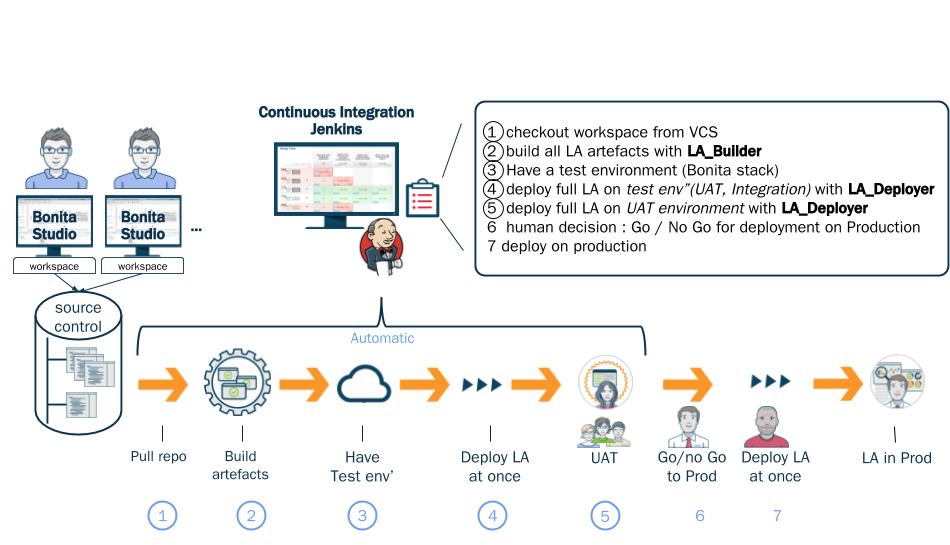
\includegraphics[width=\textwidth,keepaspectratio]{dev-to-prod.png}
\caption{Dev à Prod}
\label{fig:dev-to-prod}
\end{figure}

Les technologies utilisées actuellement sont:
\begin{itemize}
  \item Ansible
  \item Python
  \item Docker
  \item Jenkins
  \item Cloud (AWS)
\end{itemize}

Pour cette mission, j'ai dû approfondir mes connaissances sur:
\subparagraph{DevOps} De nouvelles approches qui incluent l'Intégration Continue (CI), le Déploiement Continu (CD).
\subparagraph{Agile} La communication dans un environnement agile avec ses rituels.
\subparagraph{Python} Comme un langage complet avec le paradigme OO avec TDD comme méthodologie.
\subparagraph{Docker} Les bonnes pratiques pour créer une image, et comment nous pouvons les utiliser pour déployer plus rapidement des applications.
\subparagraph{Jenkins} L’architecture et le langage DSL pour  créer des \enquote{jobs} et \enquote{pipelines} pour automatiser les tests, la compilation, l’empaquetage d'un produit final.
\subparagraph{AWS} Tous les nombreux services et la façon de nous en servir.
